\documentclass[12pt,twoside, a4paper]{article}
\usepackage[utf8]{inputenc}
\usepackage[brazil]{babel}
\usepackage[margin = 0.5in]{geometry}
\usepackage{amsmath}
\usepackage{amsthm}
\usepackage{amssymb}
\usepackage{amsthm}
\usepackage{setspace}
\usepackage[americanvoltages,fulldiodes,siunitx]{circuitikz}
\usepackage{lipsum}
\usepackage{pgfplots}
\usepackage{ifthen}
\usepackage{adjustbox}
\usepackage[section]{placeins}
\usepackage{hyperref}
\usepackage{graphicx}
\usepackage{amsmath}
\usepackage{amsthm}
\usepackage{amssymb}
\usepackage{amsthm}
\usepackage{setspace}
\usepackage[americanvoltages,fulldiodes,siunitx]{circuitikz}
\usepackage{lipsum}
\usepackage{pgfplots}
\usepackage{ifthen}
\usepackage{adjustbox}
\usepackage[section]{placeins}
\usepackage{hyperref}
\usepackage{graphicx}
\usepackage{adjustbox}
\usepackage{indentfirst}
\usepackage{float}
\usepackage{pythonhighlight}


\pgfplotsset{compat=newest}
\graphicspath{ {./images/} }
%  #1 color - optional #2 x_0 #3 y_0 #4 x_f #5 y_f #6 name - optional  #7 true if adding lines to axis
\newcommand{\drawvector} [9] [color=cyan] {
\draw[line width=1.5pt,#1,-stealth](axis cs: #2, #3)--(axis cs: #4, #5) node[anchor=south west]{$#6$};
\ifthenelse{\equal{#7}{true}}{
\draw[line width=1pt,#1, dashed](axis cs: #4, #5)--(axis cs: #4, 0) node[anchor= north west]{$#8$};
\draw[line width=1pt,#1, dashed](axis cs: #4, #5)--(axis cs: 0, #5) node[anchor=south east]{$#9$};
}
{}
}
\newcommand\deriv[2]{\frac{\mathrm d #1}{\mathrm d #2}}
\pgfplotsset{width = 10cm, compat = 1.9}

\begin{document}
\title{Quarto Relatório de Lab de Eletrônica 1}
\author{Henrique da Silva \\ henrique.pedro@ufpe.br}
\date{\today}

\maketitle
\pagenumbering{gobble}
\tableofcontents
\newpage



\input{Sections/intro}

\section{Análise preliminar}

Na análise teórica, o comportamento do circuito é considerado tanto para os grandes sinais quanto para os pequenos sinais. São utilizados modelos diferentes para cada um desses casos, conforme detalhado a seguir.

\begin{figure}[H]
    \centering
    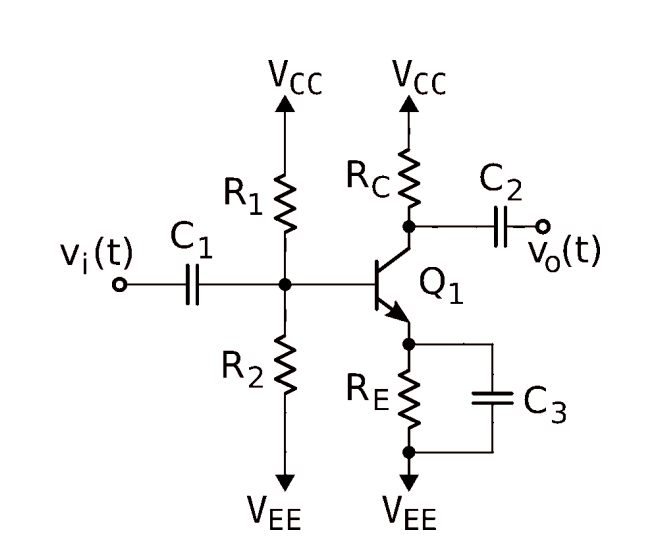
\includegraphics[width=0.5\columnwidth]{images/o_circuito.png}
    \caption{Circuito amplificador emissor de base comum.}
\end{figure}

\subsection{Análise simbólica grandes sinais}

A análise é conduzida, examinando-se as restricoes de polarizacao do transistor e as equacoes de nos do circuito.

Utiliza-se o modelo \ref{fig:modelo_grandes_sinais} para analisar o TBJ quando submetido para grandes sinais.

\begin{figure}[H]
    \centering
    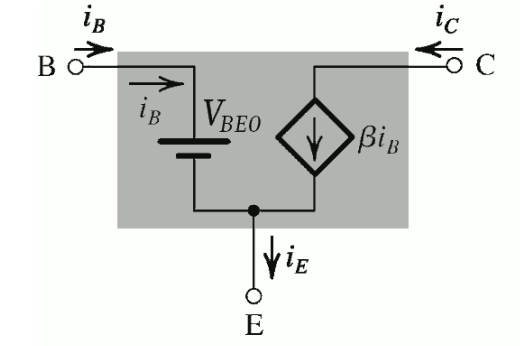
\includegraphics[width=0.5\columnwidth]{images/modelo_grandes_sinais.png}
    \caption{Modelo TBJ para grandes sinais.}
    \label{fig:modelo_grandes_sinais}
\end{figure}

Com este modelo, é possível fazer a substituição no circuito. Para grandes sinais, os capacitores do circuito se comportarão como circuito em aberto, o que permite removê-los na análise, resultando no circuito mostrado na figura \ref*{fig:circuito_grandes_sinais}.

\begin{figure}[H]
    \centering
    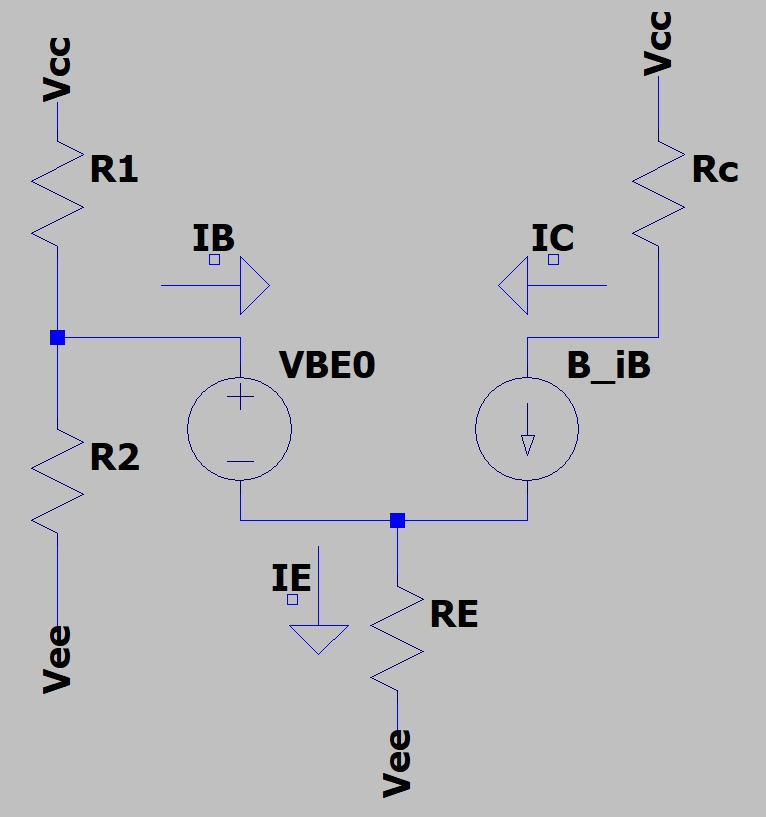
\includegraphics[width=0.3\columnwidth]{images/circuitos_grandes_sinais.png}
    \caption{Circuito com substituições para grandes sinais.}
    \label{fig:circuito_grandes_sinais}
\end{figure}

\subsubsection{Restricões}

Para que o transistor esteja na região ativa, é necessário que sejam satisfeitas as seguintes condições.

\begin{equation}
    \begin{cases}
        V_{BE} = 0.7 V  \\
        V_{CE} > 0.2 V  \\
        I_C = \beta I_B \\
        I_E = I_C + I_B
    \end{cases}
    \label{eq:restricoes_grandes_sinais}
\end{equation}

\subsubsection{Análise nodal do circuito}

Utiliza-se a lei de Kirchhoff das correntes para derivar as equações nodais seguintes.

\begin{equation}
    \begin{aligned}
         & I_{b} + \frac{V_{b} - Vee}{R_{2}} + \frac{V_{b} - Vcc}{R_{1}} = 0 \\
         & \frac{- V_{e} + Vee}{R_{e}} = I_{e}                               \\
         & \frac{- V_{c} + Vcc}{R_{c}} = I_{c}                               \\
    \end{aligned}
    \label{eq:analise_nodal_grandes_sinais}
\end{equation}

\subsubsection{Solução das tensões e correntes}

Utiliza-se as restricoes \ref*{eq:restricoes_grandes_sinais} e as equacoes do circuito \ref*{eq:analise_nodal_grandes_sinais} e resolvemos simbolicamente para $V_b$, $V_c$, $V_e$, $I_b$, $I_c$ e $I_e$.

As equações foram resolvidas utilizando a biblioteca Sympy, e o código correspondente está no apêndice. As soluções das variáveis tornaram-se muito extensas para serem representadas no formato de equações. Portanto, estamos apresentando somente as figuras que ilustram os resultados de cada variável.

\begin{figure}[H]
    \centering
    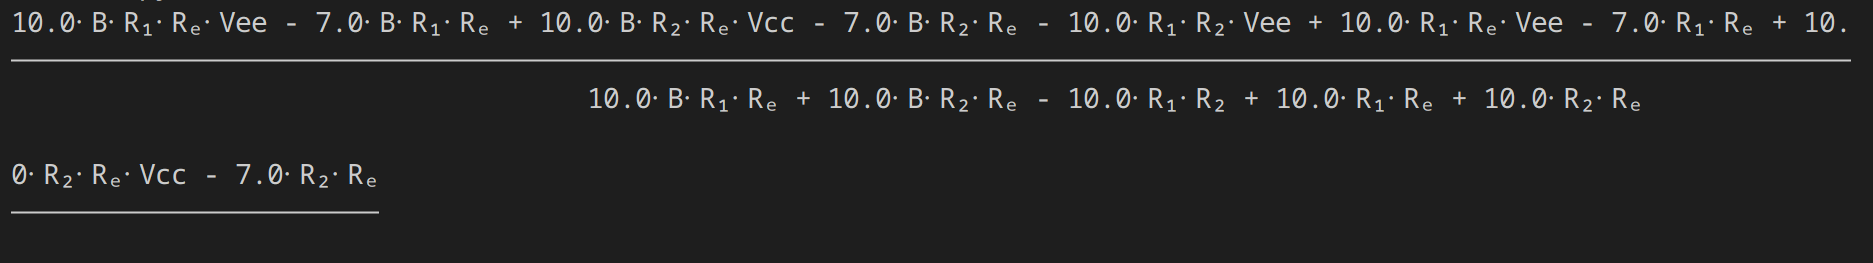
\includegraphics[width=0.7\columnwidth]{images/Ve}
    \caption{Tensão no nó $V_e$.}
\end{figure}

\begin{figure}[H]
    \centering
    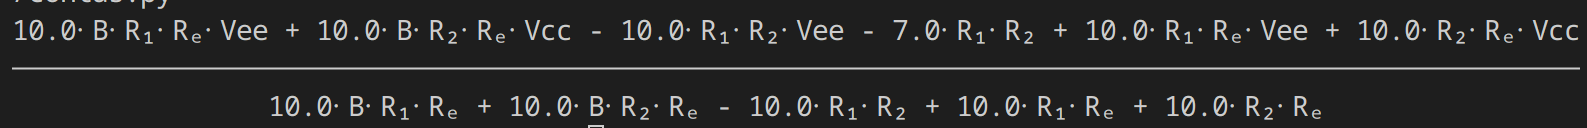
\includegraphics[width=0.7\columnwidth]{images/Vb}
    \caption{Tensão no nó $V_b$.}
\end{figure}

\begin{figure}[H]
    \centering
    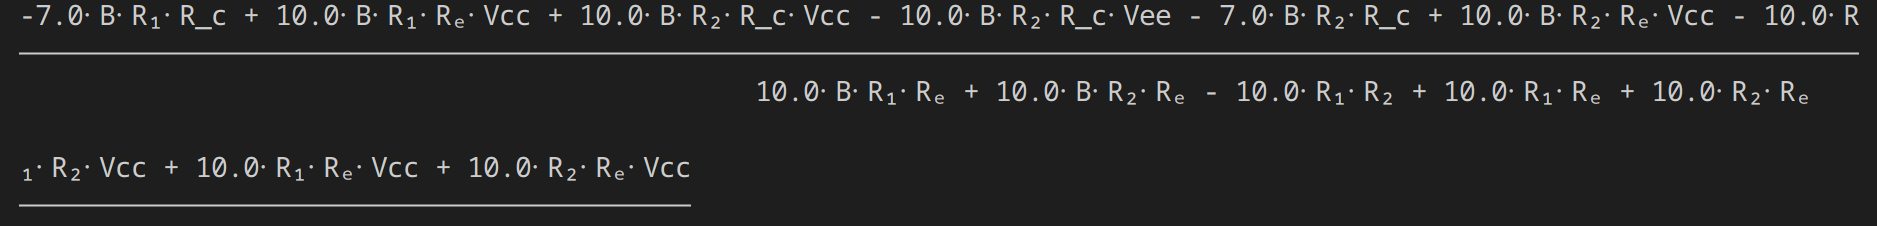
\includegraphics[width=0.7\columnwidth]{images/Vc}
    \caption{Tensão no nó $V_c$.}
\end{figure}

\begin{figure}[H]
    \centering
    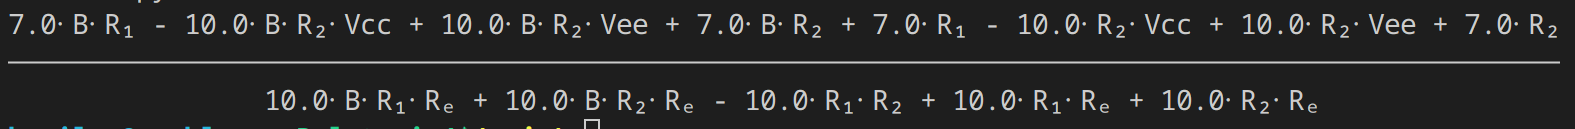
\includegraphics[width=0.7\columnwidth]{images/Ie}
    \caption{Corrente $I_e$.}
\end{figure}

\begin{figure}[H]
    \centering
    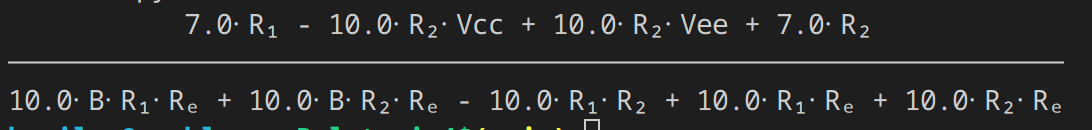
\includegraphics[width=0.7\columnwidth]{images/Ib}
    \caption{Corrente $I_b$.}
\end{figure}

\begin{figure}[H]
    \centering
    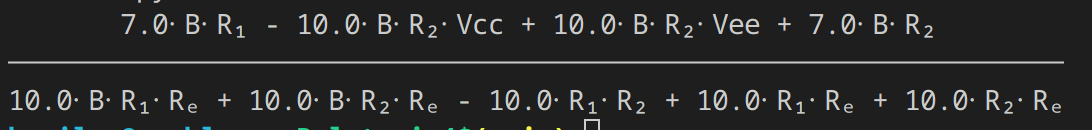
\includegraphics[width=0.7\columnwidth]{images/Ic}
    \caption{Corrente $I_c$.}
\end{figure}

\subsection{Análise simbólica pequenos sinais}

Na análise de pequenos sinais, adotamos a simplificação de considerar que os capacitores se comportam como curtos-circuitos. Além disso, assumimos que todas as fontes de tensão contínua (\emph{DC}) estão devidamente aterradas.

\begin{figure}[H]
    \centering
    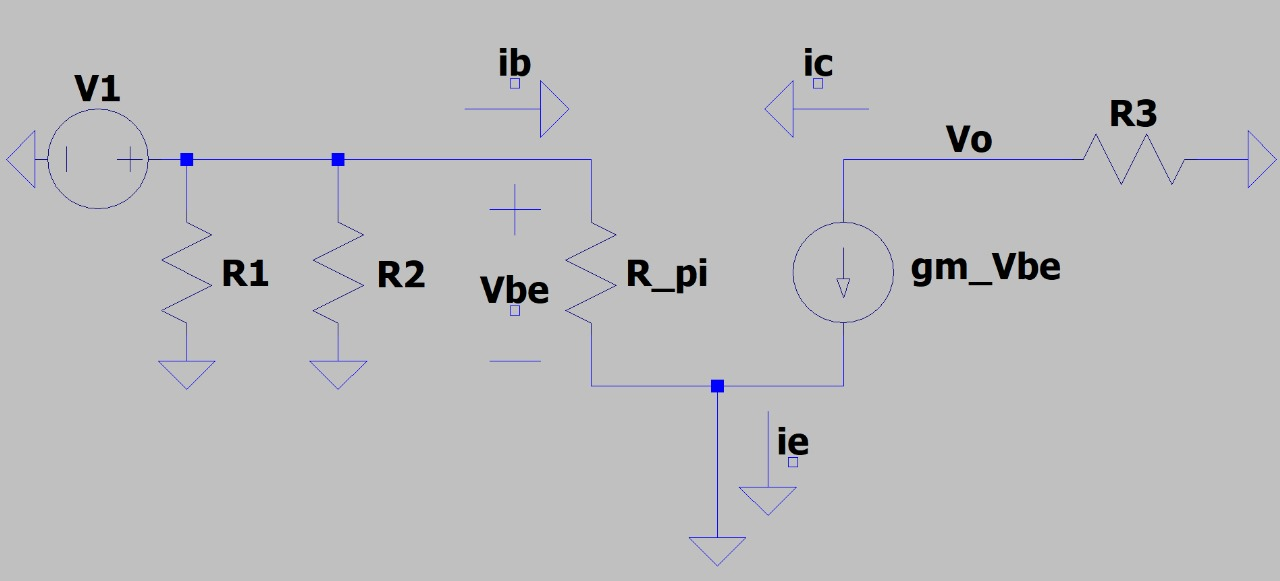
\includegraphics[width=0.6\columnwidth]{images/circuito_pequenos_sinais.png}
    \caption{Circuito com substituições para pequenos sinais.}
    \label{fig:circuito_pequenos_sinais}
\end{figure}

\subsubsection{Análise nodal do circuito}

Utiliza-se a lei de Kirchhoff das correntes para derivar as equações nodais seguintes.

\begin{equation}
    \begin{aligned}
        - I_{b} + \frac{V_{i}}{Rpi} = 0 \\
        I_{c} + \frac{V_{o}}{R_{c}} = 0 \\
        I_{c} - V_{be} gm = 0           \\
        - I_{b} - I_{c} + I_{e} = 0     \\
        I_{b} R_{\pi} - V_{be} = 0
    \end{aligned}
    \label{eq:analise_nodal_pequenos_sinais}
\end{equation}

\subsubsection{Ganho de tensão}

Para analisar o ganho de tensão, foi realizada uma solução numérica para $V_o$ e $V_i$, utilizando as equações \ref*{eq:analise_nodal_pequenos_sinais}. Os resultados obtidos são os seguintes:

\begin{equation}
    A = - gm R_c
\end{equation}

\subsubsection{Resistência de entrada}

Para analisar a resistência de entrada, foi realizada uma solução numérica para $V_i$ e $I_i$, utilizando as equações \ref*{eq:analise_nodal_pequenos_sinais}. Os resultados obtidos são os seguintes:

\begin{equation}
    R_{in} = R_{\pi}  //  R_1  //  R_2
\end{equation}

\subsubsection{Resistência de Thevenin}

Ao anular as fontes de tensão independentes, a tensão através de $R_{\pi}$ se torna zero, o que faz com que $V_{be0}$ seja igual a zero, desativando assim a fonte de corrente dependente.

Isso leva à conclusão de que a resistência de Thévenin é igual a $R_c$
.

\subsubsection{Tensão de Thevenin}

Analisa-se a tensao que esta sendo aplicada sobre $R_c$ e com isso obtemos que $V_{th} = V_o = V_c$.

\subsubsection{Constante de proporcionalidade}

Ao considerar $K = V_{th} / V_i$ e $V_{th} = V_o$, podemos afirmar que K é igual ao ganho de tensão que calculamos anteriormente.

\begin{equation}
    K = A = - gm R_c
\end{equation}


\subsection{Projeto do circuito}

Para projetar o circuito, é necessário atender aos requisitos especificados no projeto e utilizar números $n$ derivados da combinação dos \emph{CPFs} dos integrantes da equipe. No caso da equipe, todos os valores de $n$ foram $n_1 = n_2 = n_3 = n_4 = 1$. Assumindo valores como $V_{BE0} = 0,7 V$, $\beta = 350$, e $n V_r = 40 mV$, ao atender aos requisitos, é possível calcular os componentes, tensões e correntes esperadas no circuito.

\subsubsection{Componentes}

Utilizando os requisitos especificados no projeto, procede-se ao cálculo dos componentes do circuito. Esses componentes são determinados com base nas restrições e critérios estabelecidos, garantindo que o circuito atenda aos parâmetros desejados e funcione conforme o previsto.

\begin{equation}
    \begin{aligned}
         & V_{cc} - \frac{V_{cc}}{4} = (100 + 50 n_1) n V_t \\
         & V_{cc} = 8                                       \\
         & V_{ee} = -8                                      \\
    \end{aligned}
\end{equation}

\begin{equation}
    \begin{aligned}
         & R_1 = \frac{(V_{cc} - V_b)  10}{I_c} = 11 k \varOmega \\
         & R_2 = \frac{- V_{cc} - V_b}{I_c} = 2.25 k \varOmega   \\
    \end{aligned}
\end{equation}

\begin{equation}
    \begin{aligned}
         & R_c = \frac{\left(V_{cc} - \frac{V_{cc}}{4}\right)}{2 (n_2 +5)} = 500\varOmega \\
         & R_e = \frac{V_e + V_{cc}}{I_e} = 167 \varOmega
    \end{aligned}
\end{equation}

\subsubsection{Aproximações para valores comerciais}

Neste ponto do projeto, são realizadas as seguintes aproximações para os valores dos resistores, considerando as opções disponíveis no mercado de componentes eletrônicos.

\begin{center}
    \begin{tabular}{ |c|c|c| }
        \hline
        Componente & Teorico            & Comercial        \\
        $R_1$      & $11k \varOmega$    & $12k \varOmega$  \\
        $R_2$      & $2.25 k \varOmega$ & $2.2k \varOmega$ \\
        $R_c$      & $500 \varOmega$    & $470 \varOmega$  \\
        $R_e$      & $167 \varOmega$    & $180 \varOmega$  \\
        \hline
    \end{tabular}
\end{center}

\subsubsection{Tensão para grandes sinais}

Ao empregarmos os valores comerciais disponíveis, desvendamos os seguintes dados referentes às tensões e correntes de polarização que percorrem o circuito.


\begin{equation}
    \begin{aligned}
         & V_b = -5.57 V         \\
         & V_c = 3.5 V           \\
         & V_e = -6.27 V         \\
         & I_b = -2.7* 10^{-5} A \\
         & I_c = 10 mA           \\
         & I_e = 10 mA           \\
    \end{aligned}
\end{equation}

Obtem-se $V_{Rc}$ e $V_{Re}$ utilizando a lei de Ohm sobre os resistores $R_c$ e $R_e$.

\begin{equation}
    \begin{aligned}
         & V_{Rc} = 4.7 V \\
         & V_{Re} = 1.8 V
    \end{aligned}
\end{equation}

Ao alinharmos os valores das resistências com os disponíveis no mercado, constatamos que as correntes de polarização sofrem variações significativas. Essas oscilações acabam por comprometer a consecução dos requisitos previamente estipulados, desencadeando desafios adicionais no contexto do projeto do circuito.

Para contornar esse desafio, é imperativo efetuar uma modificação na resistência $R_2$, com o objetivo de amplificar a corrente $I_e$. Essa medida se faz indispensável para garantir o cumprimento dos requisitos de desempenho do circuito, pois apenas assim será possível alcançar os valores ideais de tensão e corrente de polarização necessários para o correto funcionamento do sistema.


\subsubsection{Tensão para pequenos sinais}

\section{Medições em laboratório}

Nesta seção, são apresentados os detalhes e resultados das medições realizadas no experimento, com o objetivo de obter dados quantitativos para análise e validação dos resultados teóricos previamente obtidos.

\begin{figure}[H]
    \centering
    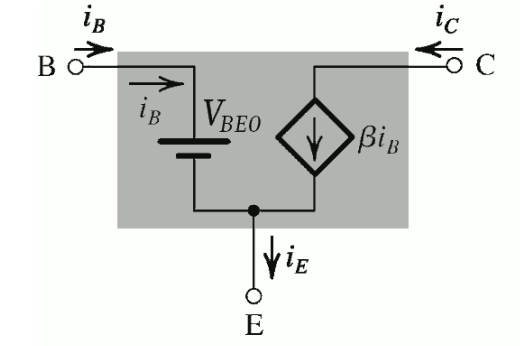
\includegraphics[width=0.5\columnwidth]{images/modelo_grandes_sinais.png}
    \caption{Circuito montado em laboratório.}
\end{figure}

\subsection{Componentes}

Os seguintes valores foram medidos para os componentes que foram empregados no circuito:

\begin{equation}
    \begin{aligned}
         & R_1 = 11743           \\
         & R_2 = 2650            \\
         & R_c = 470             \\
         & R_e = 178.4           \\
         & R_L = 145.5           \\
         & C_1 = 10.245 \mu F    \\
         & C_2 = 107.25 \mu F    \\
         & C_3 = 106 \mu F       \\
         & Potenciometro = 10.3k
    \end{aligned}
\end{equation}

\subsection{Medições de grandes sinais}

Para grandes sinais considera-se que os capacitores estao em aberto. Logo, na pratica isto implica em remover os capacitores do circuito e realizar as medicoes. Os resultados obtidos estao apresentados a seguir:

\begin{equation}
    \begin{aligned}
         & V_{cc} = 8.006  V \\
         & V_{ee} = -8.006 V \\
         & V_b = - 5.12 V    \\
         & V_e = -5.7 V      \\
         & V_c = 2.14 V      \\
         & V_{rc} = 5.87 V   \\
    \end{aligned}
\end{equation}

\subsection{Medições de pequenos sinais}

No contexto de pequenos sinais, é comum considerar que os capacitores atuam como componentes de baixa impedância, funcionando praticamente como curtos-circuitos. Portanto, na aplicação prática, essa premissa implica na inclusão dos capacitores no circuito para, em seguida, efetuarmos as medições necessárias. Nossa configuração envolve uma tensão de entrada, denotada por $V_i$, com uma amplitude de $50 mV_{pp}$ e frequência de $10 kHz$.

\subsubsection{$V_{be}$}

\begin{figure}[H]
    \centering
    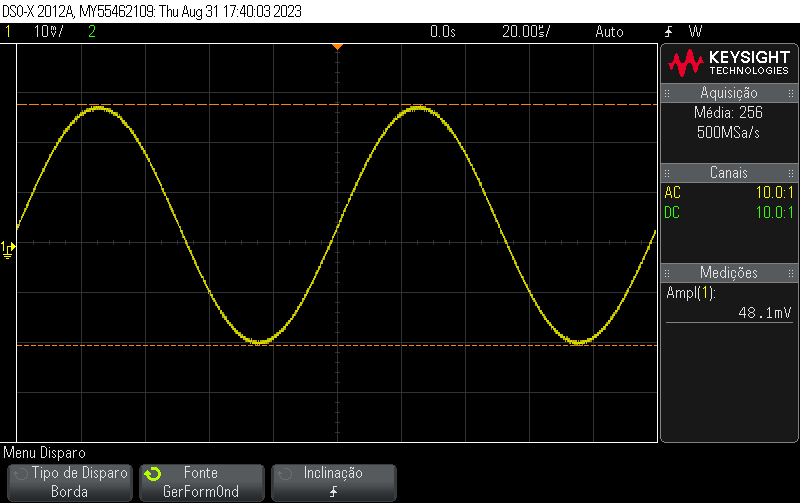
\includegraphics[width=0.5\columnwidth]{images/v_be.png}
    \caption{Tensão sobre $V_{be}$.}
\end{figure}

\subsubsection{$V_{o}$}

\begin{figure}[H]
    \centering
    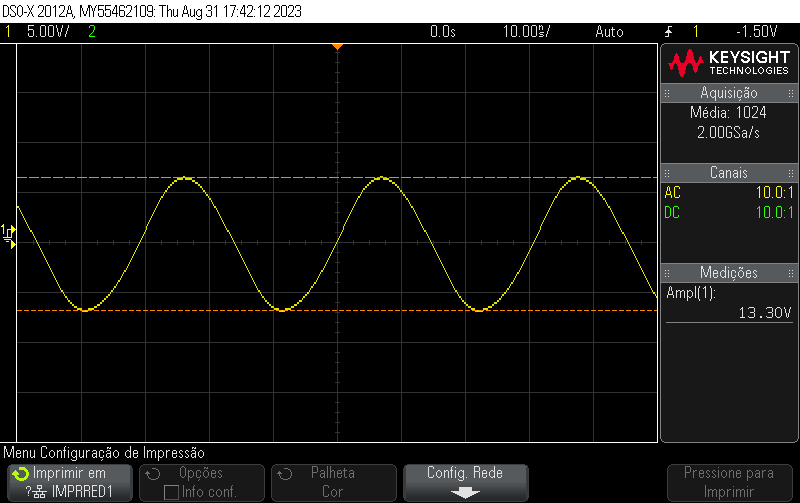
\includegraphics[width=0.5\columnwidth]{images/V_o.png}
    \caption{Tensão sobre $V_{o}$.}
\end{figure}

\subsubsection{$V_{o}$}

\begin{figure}[H]
    \centering
    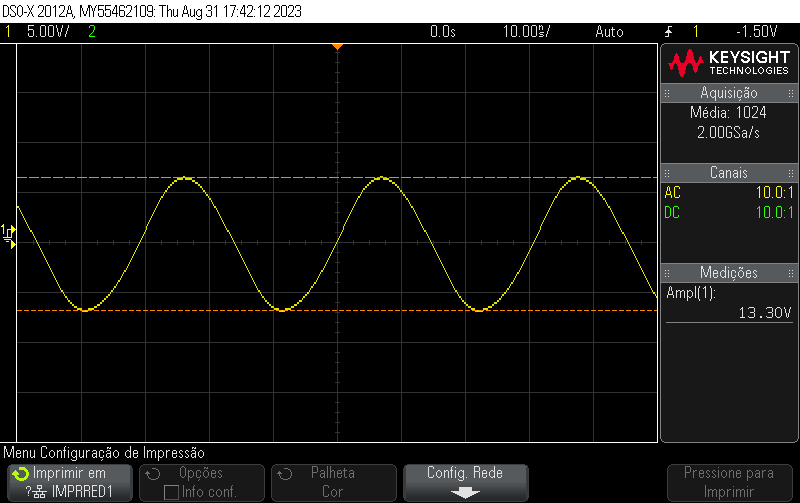
\includegraphics[width=0.5\columnwidth]{images/V_o.png}
    \caption{Tensão sobre $V_{o}$.}
\end{figure}


\subsubsection{$V_{L}$}

\begin{figure}[H]
    \centering
    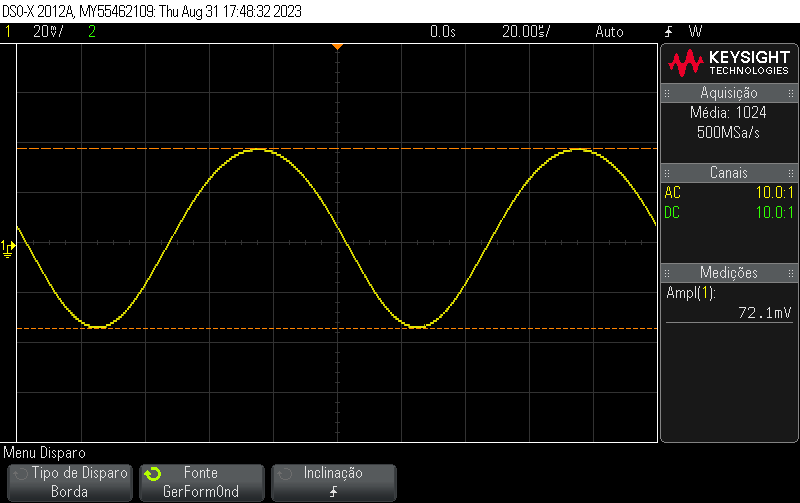
\includegraphics[width=0.5\columnwidth]{images/V_L.png}
    \caption{Tensão sobre $V_{L}$.}
\end{figure}

\subsubsection{Tensões sobre potenciometro e $R_L$}

Aqui mede-se cinco pontos de tensão sobre o potenciômetro e $R_L$ para diferentes valores de resistência do potenciômetro. Os resultados obtidos estão apresentados a seguir:

\begin{figure}[H]
    \centering
    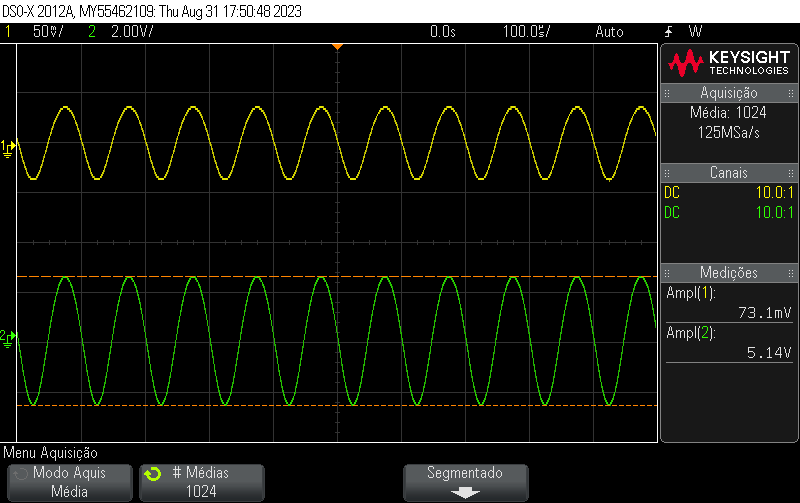
\includegraphics[width=0.5\columnwidth]{images/v_pot1.png}
    \caption{Tensão sobre $R_L$ e o potenciômetro em seu máximo.}
\end{figure}

\begin{figure}[H]
    \centering
    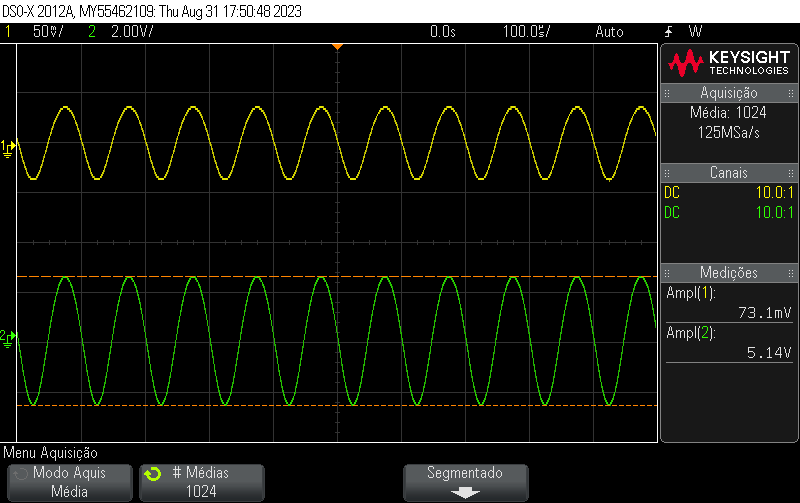
\includegraphics[width=0.5\columnwidth]{images/v_pot1.png}
    \caption{Tensão sobre $R_L$ e o potenciômetro em $75\%$ de seu máximo.}
\end{figure}

\begin{figure}[H]
    \centering
    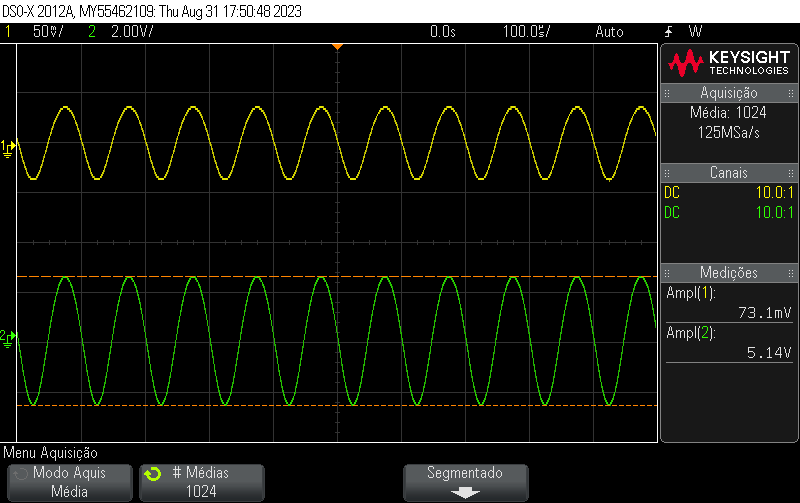
\includegraphics[width=0.5\columnwidth]{images/v_pot1.png}
    \caption{Tensão sobre $R_L$ e o potenciômetro em $50\%$ de seu máximo.}
\end{figure}

\begin{figure}[H]
    \centering
    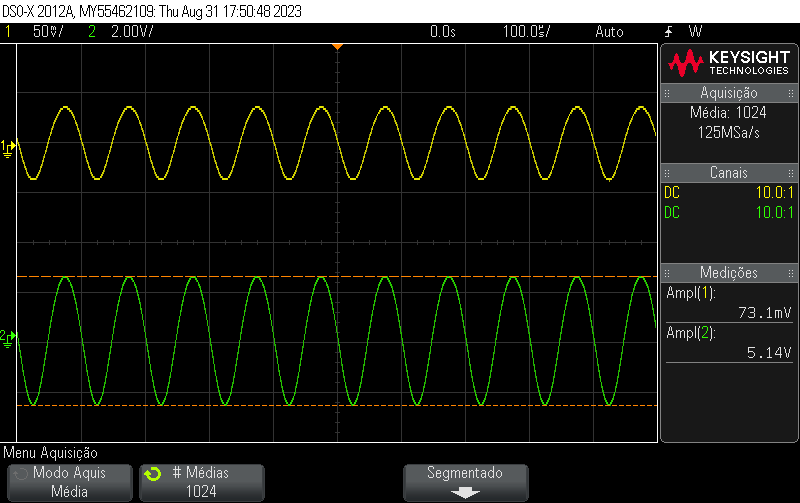
\includegraphics[width=0.5\columnwidth]{images/v_pot1.png}
    \caption{Tensão sobre $R_L$ e o potenciômetro em $25\%$ de seu máximo.}
\end{figure}

\begin{figure}[H]
    \centering
    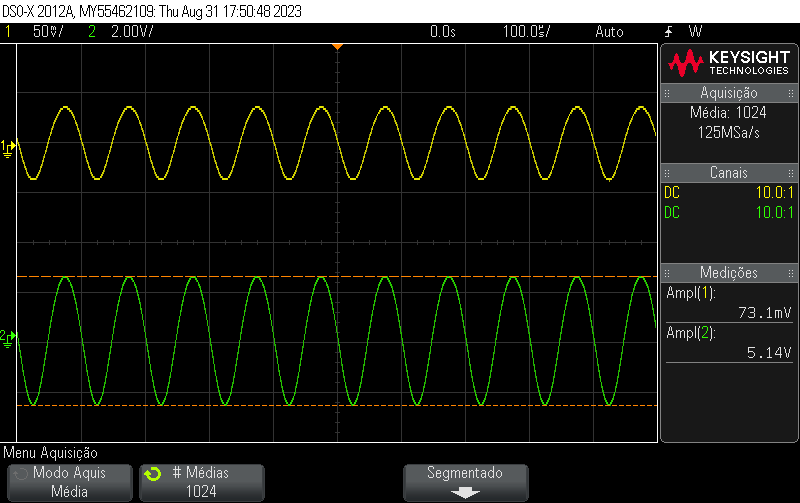
\includegraphics[width=0.5\columnwidth]{images/v_pot1.png}
    \caption{Tensão sobre $R_L$ e o potenciômetro em seu mínimo.}
\end{figure}


\section{Análise dos resultados}

Na análise, foca-se nas frequências de corte para compreender a importância de cada capacitor em sua determinação. Isso permite não apenas quantificar a influência de cada componente, mas também compreender a complexa interação entre eles.

\subsection{Frequências de corte}

Para o circuito com seus componentes inciais temos a seguinte frequência de corte:

\subsubsection{Circuito original}

\begin{equation}
    F_L = 880 Hz
\end{equation}

\subsubsection{Circuito com $C_1$ 10 vezes menor}

\begin{equation}
    F_L = 1.1 kHz
\end{equation}

\subsubsection{Circuito com $C_1$ 10 vezes maior}

\begin{equation}
    F_L = 880 Hz
\end{equation}

\subsubsection{Circuito com $C_2$ 10 vezes menor}

\begin{equation}
    F_L = 8.3 kHz
\end{equation}

\subsubsection{Circuito com $C_2$ 10 vezes maior}

\begin{equation}
    F_L = 480 Hz
\end{equation}

\subsubsection{Circuito com $C_3$ 10 vezes menor}

\begin{equation}
    F_L = 999 Hz
\end{equation}

\subsubsection{Circuito com $C_3$ 10 vezes maior}

\begin{equation}
    F_L = 870 Hz
\end{equation}

\subsection{Capacitor dominante}

Ao dispor dessas frequências, torna-se evidente que o capacitor $C_2$ desempenha um papel proeminente e determinante nas características de corte do circuito. Sua influência preponderante sugere que as propriedades específicas desse componente exercem um impacto significativo na resposta do circuito em diferentes faixas de frequência.

\section{Conclusões}

Chegamos à conclusão de que o experimento foi conduzido com êxito, apresentando resultados que se aproximaram das expectativas inicialmente estabelecidas. A análise do circuito Darlington proporcionou uma compreensão mais aprofundada do comportamento dos transistores, bem como das análises necessárias para sua polarização e controle.

Foi possível realizar a montagem do projeto e empreender uma análise específica do componente preponderante no circuito, o capacitor $C_2$. Essa análise revelou a influência significativa de $C_2$ na frequência de corte do circuito, proporcionando uma visão mais apurada de sua contribuição para o desempenho global do sistema.

\section{Apêndice}

Abaixo se encontra o código utilizado para a análise simbólica e numérica do circuito.

\begin{python}
    #from google.colab import drive
    #drive.mount('/content/drive')

    # Updating sympy to version 1.12 for faster inverse laplace transform
    # You need to restart the environment for the changes to take action
    # You need to run it before every session, or else the version will
    # be 1.11.1

    from google.colab import files

    %pip install -q --upgrade sympy

    import sympy
    sympy.__version__

    import matplotlib.pyplot as plt
    from sympy import *
    from IPython.core.interactiveshell import InteractiveShell

    # Allows multiple latex formatted lines
    InteractiveShell.ast_node_interactivity = 'all'

    # init_session prints the result in latex format, and has some useful presets,
    # more information at: https://docs.sympy.org/latest/modules/interactive.html
    init_session(quiet=True)
    # Allows the use of unicode characters
    init_printing(use_unicode=True)

\end{python}

\begin{python}
    import matplotlib.pyplot as plt
    from sympy import *

    # init_session prints the result in latex format, and has some useful presets,
    # more information at: https://docs.sympy.org/latest/modules/interactive.html
    init_session(quiet=True)
    # Allows the use of unicode characters
    init_printing(use_unicode=True)

    R0, R1, R2, R3, R4, R5, R6, R7, R8, R9, R10, R11, R12, R13 = \
    symbols('R0 R1 R2 R3 R4 R5 R6 R7 R8 R9 R10 R11 R12 R13')

    Va0, Va1, Va2, Va3, Va4, Va5, Va6, Va7, Va8, Va9, Va10 = \
    symbols('Va0 Va1 Va2 Va3 Va4 Va5 Va6 Va7 Va8 Va9 Va10')

    V0, V1, V2, V3, V4, V5, V6, V7, V8, V9, V10 = \
    symbols('V0 V1 V2 V3 V4 V5 V6 V7 V8 V9 V10')

    Vo0, Vo1, Vo2, Vo3, Vo4, Vo5, Vo6, Vo7, Vo8, Vo9, Vo10 = \
    symbols('Vo0 Vo1 Vo2 Vo3 Vo4 Vo5 Vo6 Vo7 Vo8 Vo9 Vo10')

    Vl0, Vl1, Vl2, Vl3, Vl4, Vl5, Vl6, Vl7, Vl8, Vl9, Vl10 = \
    symbols('Vl0 Vl1 Vl2 Vl3 Vl4 Vl5 Vl6 Vl7 Vl8 Vl9 Vl10')

    array_resistores = [R0, R1, R2, R3, R4, R5, R6, R7, R8, R9, R10, R11, R12, R13]

    Va = [Va0, Va1, Va2, Va3, Va4, Va5, Va6, Va7, Va8, Va9, Va10]

    V = [V0, V1, V2, V3, V4, V5, V6, V7, V8, V9, V10]

    Vo = [Vo0, Vo1, Vo2, Vo3, Vo4, Vo5, Vo6, Vo7, Vo8, Vo9, Vo10]

    Vl = [Vl0, Vl1, Vl2, Vl3, Vl4, Vl5, Vl6, Vl7, Vl8, Vl9, Vl10]

\end{python}

\begin{python}
    # Recebe um array de resistores e calcula a resistencia equivalente
    def paralelo(array_resistor, jump):
    sum = 0
    for i in range(len(array_resistor)):
    if i != jump:
    sum += 1/array_resistor[i]

    return 1/sum

    # Recebe um vetor de tensoes de entrada e um vetor de resistores ambos de mesmo tamanho e retorna o vetor com as tensoes de saida
    def divisorTensao(Vin, Vout ,resistores):
    for i in range(len(Vout)):
    Req = paralelo(resistores, i)
    Vout[i] = Vin[i]*Req/(resistores[i] + Req)
    return Vout
\end{python}

\begin{python}

    Va[0:4]=[0]*4
    Va[4:10] = divisorTensao(V[4:10], Va[4:10], array_resistores[4:10])
    Va[10] = 0
    Va

    for i in range(len(Vo)):
    if i<4:
    Vo[i]=0
    elif i<10:
    Vo[i] = Va[i]*(1 + array_resistores[11]/array_resistores[10])
    else:
    Vo[i] = -2.5*V[i]*array_resistores[11]/array_resistores[10]
    Vo

    for i in range(len(Vl)):
    if i<4:
    Vl[i] = -V[i]*array_resistores[13]/array_resistores[i]
    else:
    Vl[i] = -Vo[i]*(array_resistores[13]/array_resistores[12])
    Vl

    #K1 = R13
    #K2 = (R13/R12)(1+(R11/R10))
    #S10 = (2.5*R11*R13)/(R10*R12)

\end{python}

% \section{Anexos}

Código utilizado para geração de gráficos de bode, e análise utilizando as frequências de cortes obtidas experimentalmente.

\begin{python}
    import numpy as np
    import matplotlib.pyplot as plt
    from scipy.optimize import curve_fit



    fc1 = 210000
    fc2 = 11800


    freqs1 = np.array([0.002*fc1, 0.01*fc1, 0.05*fc1, 0.2*fc1, 0.5*fc1,
            0.8*fc1, fc1, 2*fc1, 4*fc1, 10*fc1, 20*fc1, 40*fc1])
    vin1 = np.array([0.2975, 0.297, 0.298, 0.297, 0.298,
            0.301, 0.297, 0.297, 0.3, 0.302, 0.301, 0.315])
    vout1 = np.array([1.404, 1.405, 1.403, 1.393, 1.306, 1.124,
            0.975, 0.54, 0.276, 0.114, 0.057, 0.031])


    freqs2 = np.array([0.05*fc2, 0.1*fc2, 0.2*fc2, 0.5*fc2, 0.8*fc2, fc2,
            2*fc2, 5*fc2, 20*fc2, 50*fc2, 200*fc2, 500*fc2, 1000*fc2])
    vin2 = np.array([0.1191, 0.1199, 0.12, 0.121, 0.122, 0.122,
            0.1218, 0.123, 0.123, 0.121, 0.121, 0.125, 0.151])
    vout2 = np.array([14.01, 13.95, 13.77, 12.61, 10.85, 9.8, 5.92,
            2.548, 0.645, 0.258, 0.0652, 0.0205, 0.0122])




    def mag_sqr_fun(f, K, fc):
    return (K*fc)**2/(f**2 + fc**2)


    def dB(m):
    return 20*np.log10(m)




    (K1, fc1), _ = curve_fit(lambda f, K, fc: dB(mag_sqr_fun(f, K, fc)),
    freqs1, 2*dB(vout1/vin1))


    print(f"""O ganho K eh {round(K1, 1)}
    A frequencia de corte eh {round(fc1, 1)} Hz""")

    f1 = np.logspace(np.log10(freqs1[0]) - 1, np.log10(freqs1[-1]) + 0.3)
    mag1 = dB(mag_sqr_fun(f1, K1, fc1))/2

    plt.semilogx(f1, mag1)
    plt.semilogx(freqs1, dB(vout1/vin1), "*")
    plt.xlabel("Freq (Hz)")
    plt.ylabel("Mag(H) (dB)")
    plt.title("Grafico de Bode de magnitude para o 1 circuito")
    plt.grid()
    plt.savefig("figura1.png")
    plt.show()



    (K2, fc2), _ = curve_fit(lambda f, K, fc: dB(mag_sqr_fun(f, K, fc)),
    freqs2, 2*dB(vout2/vin2))

    print("\n\nResultados para o 2 circuito:\n")
    print(f"""O ganho K eh {round(K2, 1)}
    A frequencia de corte eh {round(fc2, 1)} Hz""")

    f2 = np.logspace(np.log10(freqs2[0]) - 1, np.log10(freqs2[-1]) + 0.3)
    mag2 = dB(mag_sqr_fun(f2, K2, fc2))/2

    plt.semilogx(f2, mag2)
    plt.semilogx(freqs2, dB(vout2/vin2), "*")
    plt.xlabel("Freq (Hz)")
    plt.ylabel("Mag(H) (dB)")
    plt.title("Grafico de Bode de magnitude para o 2 circuito")
    plt.grid()
    plt.savefig("figura2.png")
    plt.show()




    plt.semilogx(f1, mag1)
    plt.semilogx(f2, mag2)
    plt.semilogx(freqs1, dB(vout1/vin1), "*")
    plt.semilogx(freqs2, dB(vout2/vin2), "*")
    plt.xlabel("Freq (Hz)")
    plt.ylabel("Mag(H) (dB)")
    plt.title("Grafico de Bode de magnitude para ambos os circuitos")
    plt.grid()
    plt.savefig("figura3.png")
    plt.show()

\end{python}


\end{document}